% !TeX program = xelatex
\documentclass{article}
\usepackage[a4paper,top=11mm,bottom=10mm,left=12.7mm,right=12.7mm]{geometry}
\usepackage{fontspec}
\usepackage{xcolor}
\usepackage{tikz}
\usetikzlibrary{arrows.meta,bending,shapes.geometric}
\usepackage{ragged2e}
\pagestyle{empty}
\setlength{\parindent}{0pt}
\setlength{\parskip}{0pt}
\hyphenpenalty=10000
\exhyphenpenalty=10000
\emergencystretch=3em
\setmainfont{SourceSans3}[Path=fonts/, Extension=.otf, UprightFont=*-Regular, BoldFont=*-Bold]
\renewcommand\normalsize{\fontsize{13}{19}\selectfont}
\newcommand\klein{\fontsize{11}{14}\selectfont}
\definecolor{ink}{HTML}{1F1D1A}
\definecolor{kopf}{HTML}{E6E6E6}
\definecolor{feld}{HTML}{C8C8C8}
\definecolor{gitter}{HTML}{B4B4B4}
\newcommand\titel[1]{{\bfseries\fontsize{28}{30}\selectfont #1\par}\vspace{2.5mm}\hrule height 1.2pt\vspace{4mm}}
\newcommand\aufgabe[2]{\par\noindent\begin{tikzpicture}[baseline=(n.base)]
  \node[circle,fill=ink,text=white,minimum size=7mm,inner sep=0,font=\bfseries\fontsize{12}{12}\selectfont] (n) {#1};
  \end{tikzpicture}\hspace{2.5mm}\textbf{#2}\par\vspace{2.5mm}}
\newcommand\stern{\tikz[baseline=-0.6ex]{\node[circle,fill=ink,inner sep=0pt,minimum size=7mm]{};\node[star,star points=5,star point ratio=2.3,fill=white,inner sep=0pt,minimum size=4.4mm]{};}}
\newcommand\linie[1]{\tikz[baseline=0pt]\draw[line width=0.8pt,draw=ink] (0,-0.9mm) -- (#1,-0.9mm);}
\AtBeginDocument{\normalsize\RaggedRight\color{ink}}
\begin{document}
\titel{Zweisatz und Dreisatz}
\aufgabe{1}{Ergänze beide Rechenpfeile und den fehlenden Wert.}
Im Schreibwarenladen kosten 4 Ordner 6~€. Tom kauft 8 Ordner, Lea 2 Ordner.\par\vspace{4mm}
\noindent
\begin{tikzpicture}[x=1mm,y=1mm,baseline=0pt]
\useasboundingbox (0,-1.5) rectangle (184.6,4);
\node[anchor=base west,inner sep=0] at (0,0) {Zuordnung:};
\draw[line width=0.8pt,draw=ink] (27.7,-0.9) -- (97.7,-0.9);
\draw[line width=0.8pt,draw=ink] (114.6,-0.9) -- (184.6,-0.9);
\node[anchor=base,inner sep=0,font=\fontsize{14}{17}\selectfont] at (62.7,0) {Anzahl der Ordner};
\node[anchor=base,inner sep=0,font=\fontsize{14}{17}\selectfont] at (149.6,0) {Preis in €};
\node[anchor=base west,inner sep=0] at (103.1,0) {\fontsize{17.2}{17}\selectfont$\rightarrow$};
\end{tikzpicture}\par\vspace{3mm}
\noindent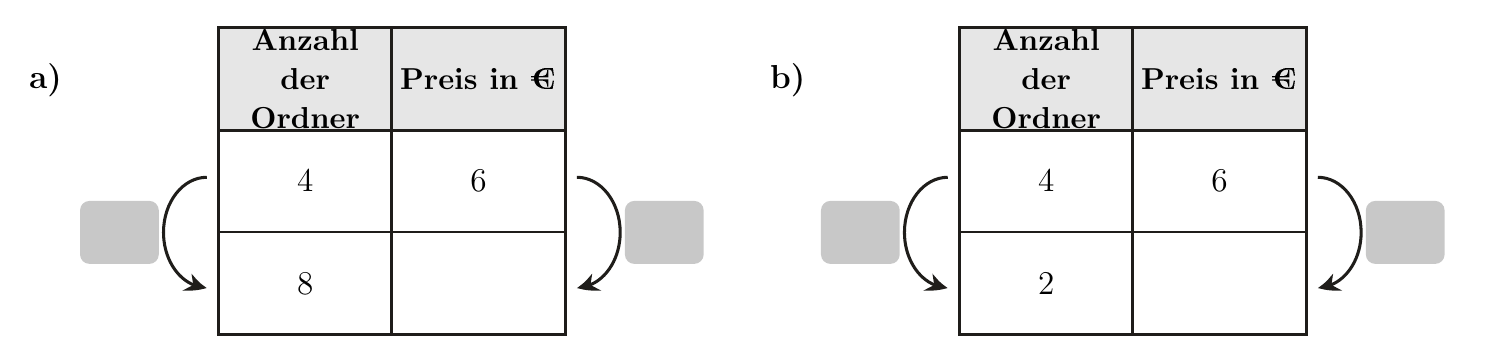
\begin{tikzpicture}[line width=1.1pt,draw=ink,x=1mm,y=1mm]
\useasboundingbox (0,0) rectangle (184.6,-39);
\node[anchor=north west,inner sep=0,font=\bfseries] at (0,-4.4) {a)};
\node[anchor=north west,inner sep=0,font=\bfseries] at (94.1,-4.4) {b)};
\fill[kopf] (24.25,0) rectangle (68.25,-13);
\draw (24.25,0) rectangle (68.25,-39);
\draw (46.25,0) -- (46.25,-39);
\draw (24.25,-13) -- (68.25,-13);
\draw[line width=0.7pt] (24.25,-26) -- (68.25,-26);
\node[text width=20mm,align=center,font=\bfseries\klein] at (35.25,-6.5) {Anzahl der Ordner};
\node[text width=20mm,align=center,font=\bfseries\klein] at (57.25,-6.5) {Preis in €};
\node at (35.25,-19.5) {4};
\node at (57.25,-19.5) {6};
\node at (35.25,-32.5) {8};
\draw[-{Stealth[length=2.6mm,width=2.4mm,bend]}] (22.75,-19.00) arc[start angle=90,end angle=270,x radius=5.5,y radius=7.00];
\fill[feld,rounded corners=1.2mm] (6.649999999999999,-30.00) rectangle (16.65,-22.00);
\draw[-{Stealth[length=2.6mm,width=2.4mm,bend]}] (69.75,-19.00) arc[start angle=90,end angle=-90,x radius=5.5,y radius=7.00];
\fill[feld,rounded corners=1.2mm] (75.85,-30.00) rectangle (85.85,-22.00);
\fill[kopf] (118.35,0) rectangle (162.35,-13);
\draw (118.35,0) rectangle (162.35,-39);
\draw (140.35,0) -- (140.35,-39);
\draw (118.35,-13) -- (162.35,-13);
\draw[line width=0.7pt] (118.35,-26) -- (162.35,-26);
\node[text width=20mm,align=center,font=\bfseries\klein] at (129.35,-6.5) {Anzahl der Ordner};
\node[text width=20mm,align=center,font=\bfseries\klein] at (151.35,-6.5) {Preis in €};
\node at (129.35,-19.5) {4};
\node at (151.35,-19.5) {6};
\node at (129.35,-32.5) {2};
\draw[-{Stealth[length=2.6mm,width=2.4mm,bend]}] (116.85,-19.00) arc[start angle=90,end angle=270,x radius=5.5,y radius=7.00];
\fill[feld,rounded corners=1.2mm] (100.75,-30.00) rectangle (110.75,-22.00);
\draw[-{Stealth[length=2.6mm,width=2.4mm,bend]}] (163.85,-19.00) arc[start angle=90,end angle=-90,x radius=5.5,y radius=7.00];
\fill[feld,rounded corners=1.2mm] (169.95,-30.00) rectangle (179.95,-22.00);
\end{tikzpicture}\par
\vspace{5mm}
\aufgabe{2}{Schreibe die Zuordnung auf. Rechne zuerst auf 1, dann zum gesuchten Wert.}
\noindent\begin{minipage}[t]{89mm}\textbf{a)} Im Schreibwarenladen kosten 8 Hefte 20~€.\\Wie viel kosten 3 Hefte?\end{minipage}\hfill\begin{minipage}[t]{90.5mm}\textbf{b)} Im Supermarkt kosten 6 Hefte 9~€.\\Wie viel kosten 14 Hefte?\end{minipage}\par\vspace{4mm}
\noindent
\begin{tikzpicture}[x=1mm,y=1mm,baseline=0pt]
\useasboundingbox (0,-1.5) rectangle (184.6,4);
\node[anchor=base west,inner sep=0] at (0,0) {Zuordnung:};
\draw[line width=0.8pt,draw=ink] (27.7,-0.9) -- (97.7,-0.9);
\draw[line width=0.8pt,draw=ink] (114.6,-0.9) -- (184.6,-0.9);
\node[anchor=base,inner sep=0,font=\fontsize{14}{17}\selectfont] at (62.7,0) {};
\node[anchor=base,inner sep=0,font=\fontsize{14}{17}\selectfont] at (149.6,0) {};
\node[anchor=base west,inner sep=0] at (103.1,0) {\fontsize{17.2}{17}\selectfont$\rightarrow$};
\end{tikzpicture}\par\vspace{3mm}
\noindent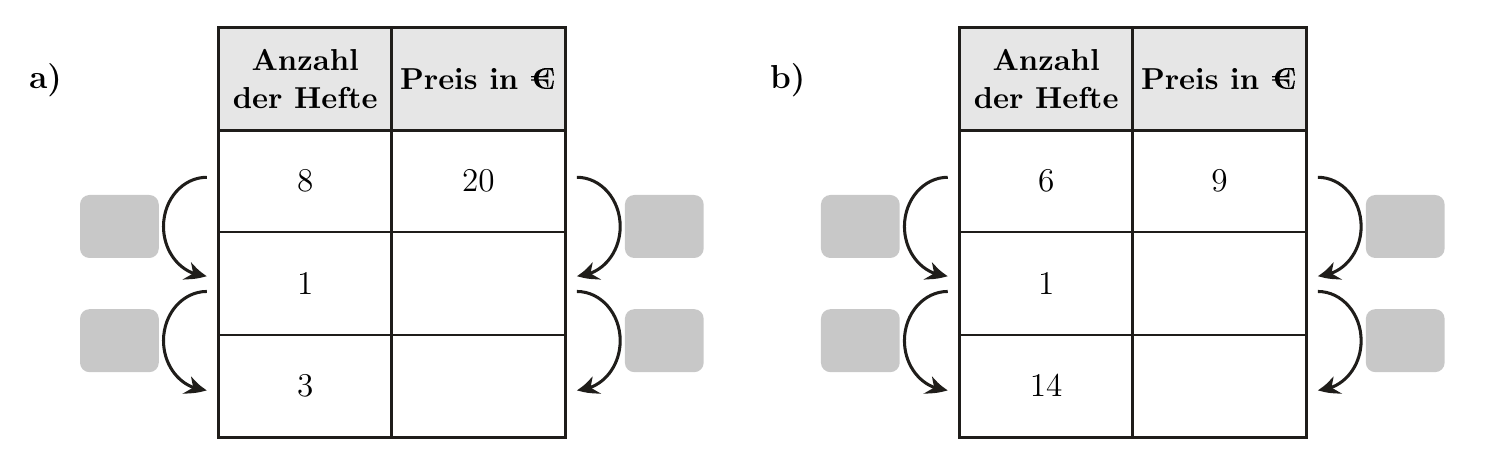
\begin{tikzpicture}[line width=1.1pt,draw=ink,x=1mm,y=1mm]
\useasboundingbox (0,0) rectangle (184.6,-52);
\node[anchor=north west,inner sep=0,font=\bfseries] at (0,-4.4) {a)};
\node[anchor=north west,inner sep=0,font=\bfseries] at (94.1,-4.4) {b)};
\fill[kopf] (24.25,0) rectangle (68.25,-13);
\draw (24.25,0) rectangle (68.25,-52);
\draw (46.25,0) -- (46.25,-52);
\draw (24.25,-13) -- (68.25,-13);
\draw[line width=0.7pt] (24.25,-26) -- (68.25,-26);
\draw[line width=0.7pt] (24.25,-39) -- (68.25,-39);
\node[text width=20mm,align=center,font=\bfseries\klein] at (35.25,-6.5) {Anzahl der Hefte};
\node[text width=20mm,align=center,font=\bfseries\klein] at (57.25,-6.5) {Preis in €};
\node at (35.25,-19.5) {8};
\node at (57.25,-19.5) {20};
\node at (35.25,-32.5) {1};
\node at (35.25,-45.5) {3};
\draw[-{Stealth[length=2.6mm,width=2.4mm,bend]}] (22.75,-19.00) arc[start angle=90,end angle=270,x radius=5.5,y radius=6.25];
\fill[feld,rounded corners=1.2mm] (6.649999999999999,-29.25) rectangle (16.65,-21.25);
\draw[-{Stealth[length=2.6mm,width=2.4mm,bend]}] (22.75,-33.50) arc[start angle=90,end angle=270,x radius=5.5,y radius=6.25];
\fill[feld,rounded corners=1.2mm] (6.649999999999999,-43.75) rectangle (16.65,-35.75);
\draw[-{Stealth[length=2.6mm,width=2.4mm,bend]}] (69.75,-19.00) arc[start angle=90,end angle=-90,x radius=5.5,y radius=6.25];
\fill[feld,rounded corners=1.2mm] (75.85,-29.25) rectangle (85.85,-21.25);
\draw[-{Stealth[length=2.6mm,width=2.4mm,bend]}] (69.75,-33.50) arc[start angle=90,end angle=-90,x radius=5.5,y radius=6.25];
\fill[feld,rounded corners=1.2mm] (75.85,-43.75) rectangle (85.85,-35.75);
\fill[kopf] (118.35,0) rectangle (162.35,-13);
\draw (118.35,0) rectangle (162.35,-52);
\draw (140.35,0) -- (140.35,-52);
\draw (118.35,-13) -- (162.35,-13);
\draw[line width=0.7pt] (118.35,-26) -- (162.35,-26);
\draw[line width=0.7pt] (118.35,-39) -- (162.35,-39);
\node[text width=20mm,align=center,font=\bfseries\klein] at (129.35,-6.5) {Anzahl der Hefte};
\node[text width=20mm,align=center,font=\bfseries\klein] at (151.35,-6.5) {Preis in €};
\node at (129.35,-19.5) {6};
\node at (151.35,-19.5) {9};
\node at (129.35,-32.5) {1};
\node at (129.35,-45.5) {14};
\draw[-{Stealth[length=2.6mm,width=2.4mm,bend]}] (116.85,-19.00) arc[start angle=90,end angle=270,x radius=5.5,y radius=6.25];
\fill[feld,rounded corners=1.2mm] (100.75,-29.25) rectangle (110.75,-21.25);
\draw[-{Stealth[length=2.6mm,width=2.4mm,bend]}] (116.85,-33.50) arc[start angle=90,end angle=270,x radius=5.5,y radius=6.25];
\fill[feld,rounded corners=1.2mm] (100.75,-43.75) rectangle (110.75,-35.75);
\draw[-{Stealth[length=2.6mm,width=2.4mm,bend]}] (163.85,-19.00) arc[start angle=90,end angle=-90,x radius=5.5,y radius=6.25];
\fill[feld,rounded corners=1.2mm] (169.95,-29.25) rectangle (179.95,-21.25);
\draw[-{Stealth[length=2.6mm,width=2.4mm,bend]}] (163.85,-33.50) arc[start angle=90,end angle=-90,x radius=5.5,y radius=6.25];
\fill[feld,rounded corners=1.2mm] (169.95,-43.75) rectangle (179.95,-35.75);
\end{tikzpicture}\par
\vspace{5mm}
\aufgabe{3}{Schreibe die Zuordnung auf. Trage die 1 selbst ein und rechne.}
\noindent\begin{minipage}[t]{89mm}\textbf{a)} Ein Auto fährt mit 6 Litern Benzin 84~km.\\Wie weit kommt es mit 4 Litern?\end{minipage}\hfill\begin{minipage}[t]{90.5mm}\textbf{b)} Ein Roller fährt mit 3 Litern Benzin 105~km.\\Wie weit kommt er mit 8 Litern?\end{minipage}\par\vspace{4mm}
\noindent
\begin{tikzpicture}[x=1mm,y=1mm,baseline=0pt]
\useasboundingbox (0,-1.5) rectangle (184.6,4);
\node[anchor=base west,inner sep=0] at (0,0) {Zuordnung:};
\draw[line width=0.8pt,draw=ink] (27.7,-0.9) -- (97.7,-0.9);
\draw[line width=0.8pt,draw=ink] (114.6,-0.9) -- (184.6,-0.9);
\node[anchor=base,inner sep=0,font=\fontsize{14}{17}\selectfont] at (62.7,0) {};
\node[anchor=base,inner sep=0,font=\fontsize{14}{17}\selectfont] at (149.6,0) {};
\node[anchor=base west,inner sep=0] at (103.1,0) {\fontsize{17.2}{17}\selectfont$\rightarrow$};
\end{tikzpicture}\par\vspace{3mm}
\noindent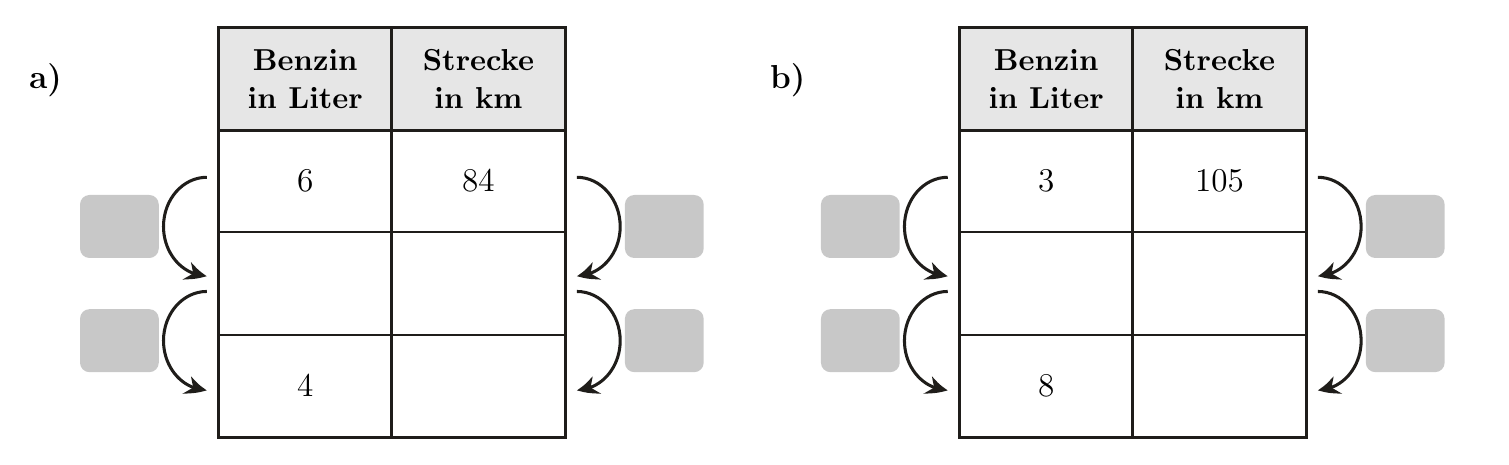
\begin{tikzpicture}[line width=1.1pt,draw=ink,x=1mm,y=1mm]
\useasboundingbox (0,0) rectangle (184.6,-52);
\node[anchor=north west,inner sep=0,font=\bfseries] at (0,-4.4) {a)};
\node[anchor=north west,inner sep=0,font=\bfseries] at (94.1,-4.4) {b)};
\fill[kopf] (24.25,0) rectangle (68.25,-13);
\draw (24.25,0) rectangle (68.25,-52);
\draw (46.25,0) -- (46.25,-52);
\draw (24.25,-13) -- (68.25,-13);
\draw[line width=0.7pt] (24.25,-26) -- (68.25,-26);
\draw[line width=0.7pt] (24.25,-39) -- (68.25,-39);
\node[text width=20mm,align=center,font=\bfseries\klein] at (35.25,-6.5) {Benzin in Liter};
\node[text width=20mm,align=center,font=\bfseries\klein] at (57.25,-6.5) {Strecke in km};
\node at (35.25,-19.5) {6};
\node at (57.25,-19.5) {84};
\node at (35.25,-45.5) {4};
\draw[-{Stealth[length=2.6mm,width=2.4mm,bend]}] (22.75,-19.00) arc[start angle=90,end angle=270,x radius=5.5,y radius=6.25];
\fill[feld,rounded corners=1.2mm] (6.649999999999999,-29.25) rectangle (16.65,-21.25);
\draw[-{Stealth[length=2.6mm,width=2.4mm,bend]}] (22.75,-33.50) arc[start angle=90,end angle=270,x radius=5.5,y radius=6.25];
\fill[feld,rounded corners=1.2mm] (6.649999999999999,-43.75) rectangle (16.65,-35.75);
\draw[-{Stealth[length=2.6mm,width=2.4mm,bend]}] (69.75,-19.00) arc[start angle=90,end angle=-90,x radius=5.5,y radius=6.25];
\fill[feld,rounded corners=1.2mm] (75.85,-29.25) rectangle (85.85,-21.25);
\draw[-{Stealth[length=2.6mm,width=2.4mm,bend]}] (69.75,-33.50) arc[start angle=90,end angle=-90,x radius=5.5,y radius=6.25];
\fill[feld,rounded corners=1.2mm] (75.85,-43.75) rectangle (85.85,-35.75);
\fill[kopf] (118.35,0) rectangle (162.35,-13);
\draw (118.35,0) rectangle (162.35,-52);
\draw (140.35,0) -- (140.35,-52);
\draw (118.35,-13) -- (162.35,-13);
\draw[line width=0.7pt] (118.35,-26) -- (162.35,-26);
\draw[line width=0.7pt] (118.35,-39) -- (162.35,-39);
\node[text width=20mm,align=center,font=\bfseries\klein] at (129.35,-6.5) {Benzin in Liter};
\node[text width=20mm,align=center,font=\bfseries\klein] at (151.35,-6.5) {Strecke in km};
\node at (129.35,-19.5) {3};
\node at (151.35,-19.5) {105};
\node at (129.35,-45.5) {8};
\draw[-{Stealth[length=2.6mm,width=2.4mm,bend]}] (116.85,-19.00) arc[start angle=90,end angle=270,x radius=5.5,y radius=6.25];
\fill[feld,rounded corners=1.2mm] (100.75,-29.25) rectangle (110.75,-21.25);
\draw[-{Stealth[length=2.6mm,width=2.4mm,bend]}] (116.85,-33.50) arc[start angle=90,end angle=270,x radius=5.5,y radius=6.25];
\fill[feld,rounded corners=1.2mm] (100.75,-43.75) rectangle (110.75,-35.75);
\draw[-{Stealth[length=2.6mm,width=2.4mm,bend]}] (163.85,-19.00) arc[start angle=90,end angle=-90,x radius=5.5,y radius=6.25];
\fill[feld,rounded corners=1.2mm] (169.95,-29.25) rectangle (179.95,-21.25);
\draw[-{Stealth[length=2.6mm,width=2.4mm,bend]}] (163.85,-33.50) arc[start angle=90,end angle=-90,x radius=5.5,y radius=6.25];
\fill[feld,rounded corners=1.2mm] (169.95,-43.75) rectangle (179.95,-35.75);
\end{tikzpicture}\par
\newpage
\aufgabe{4}{Schreibe die Zuordnung auf. Beschrifte die Tabelle, trage die Werte ein und rechne.}
Auf dem Wochenmarkt kaufen Frau Kaya und Herr Becker ein.\par\vspace{2mm}
\noindent\begin{minipage}[t]{89mm}\textbf{a)} 3~kg Äpfel kosten 7,50~€.\\Wie viel kosten 5~kg Äpfel?\end{minipage}\hfill\begin{minipage}[t]{90.5mm}\textbf{b)} 6 Gläser Honig kosten 27~€.\\Wie viel kosten 4 Gläser Honig?\end{minipage}\par\vspace{4mm}
\noindent
\begin{tikzpicture}[x=1mm,y=1mm,baseline=0pt]
\useasboundingbox (0,-1.5) rectangle (184.6,4);
\node[anchor=base west,inner sep=0] at (0,0) {Zuordnung:};
\draw[line width=0.8pt,draw=ink] (27.7,-0.9) -- (97.7,-0.9);
\draw[line width=0.8pt,draw=ink] (114.6,-0.9) -- (184.6,-0.9);
\node[anchor=base,inner sep=0,font=\fontsize{14}{17}\selectfont] at (62.7,0) {};
\node[anchor=base,inner sep=0,font=\fontsize{14}{17}\selectfont] at (149.6,0) {};
\node[anchor=base west,inner sep=0] at (103.1,0) {\fontsize{17.2}{17}\selectfont$\rightarrow$};
\end{tikzpicture}\par\vspace{3mm}
\noindent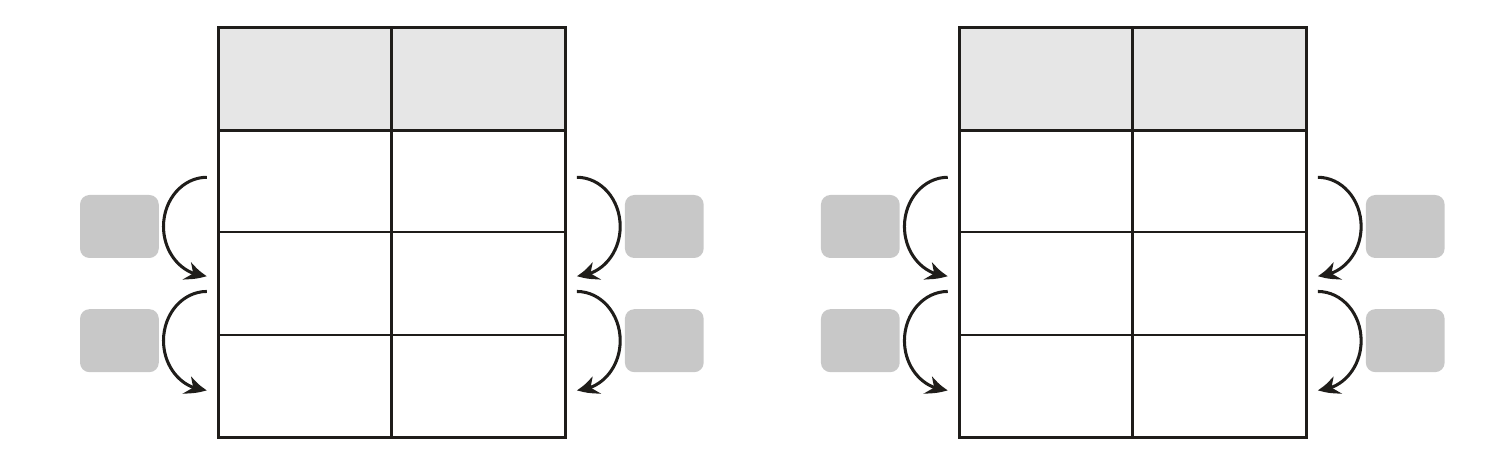
\begin{tikzpicture}[line width=1.1pt,draw=ink,x=1mm,y=1mm]
\useasboundingbox (0,0) rectangle (184.6,-52);
\fill[kopf] (24.25,0) rectangle (68.25,-13);
\draw (24.25,0) rectangle (68.25,-52);
\draw (46.25,0) -- (46.25,-52);
\draw (24.25,-13) -- (68.25,-13);
\draw[line width=0.7pt] (24.25,-26) -- (68.25,-26);
\draw[line width=0.7pt] (24.25,-39) -- (68.25,-39);
\draw[-{Stealth[length=2.6mm,width=2.4mm,bend]}] (22.75,-19.00) arc[start angle=90,end angle=270,x radius=5.5,y radius=6.25];
\fill[feld,rounded corners=1.2mm] (6.649999999999999,-29.25) rectangle (16.65,-21.25);
\draw[-{Stealth[length=2.6mm,width=2.4mm,bend]}] (22.75,-33.50) arc[start angle=90,end angle=270,x radius=5.5,y radius=6.25];
\fill[feld,rounded corners=1.2mm] (6.649999999999999,-43.75) rectangle (16.65,-35.75);
\draw[-{Stealth[length=2.6mm,width=2.4mm,bend]}] (69.75,-19.00) arc[start angle=90,end angle=-90,x radius=5.5,y radius=6.25];
\fill[feld,rounded corners=1.2mm] (75.85,-29.25) rectangle (85.85,-21.25);
\draw[-{Stealth[length=2.6mm,width=2.4mm,bend]}] (69.75,-33.50) arc[start angle=90,end angle=-90,x radius=5.5,y radius=6.25];
\fill[feld,rounded corners=1.2mm] (75.85,-43.75) rectangle (85.85,-35.75);
\fill[kopf] (118.35,0) rectangle (162.35,-13);
\draw (118.35,0) rectangle (162.35,-52);
\draw (140.35,0) -- (140.35,-52);
\draw (118.35,-13) -- (162.35,-13);
\draw[line width=0.7pt] (118.35,-26) -- (162.35,-26);
\draw[line width=0.7pt] (118.35,-39) -- (162.35,-39);
\draw[-{Stealth[length=2.6mm,width=2.4mm,bend]}] (116.85,-19.00) arc[start angle=90,end angle=270,x radius=5.5,y radius=6.25];
\fill[feld,rounded corners=1.2mm] (100.75,-29.25) rectangle (110.75,-21.25);
\draw[-{Stealth[length=2.6mm,width=2.4mm,bend]}] (116.85,-33.50) arc[start angle=90,end angle=270,x radius=5.5,y radius=6.25];
\fill[feld,rounded corners=1.2mm] (100.75,-43.75) rectangle (110.75,-35.75);
\draw[-{Stealth[length=2.6mm,width=2.4mm,bend]}] (163.85,-19.00) arc[start angle=90,end angle=-90,x radius=5.5,y radius=6.25];
\fill[feld,rounded corners=1.2mm] (169.95,-29.25) rectangle (179.95,-21.25);
\draw[-{Stealth[length=2.6mm,width=2.4mm,bend]}] (163.85,-33.50) arc[start angle=90,end angle=-90,x radius=5.5,y radius=6.25];
\fill[feld,rounded corners=1.2mm] (169.95,-43.75) rectangle (179.95,-35.75);
\end{tikzpicture}\par
\vspace{5mm}
\noindent\begin{minipage}[t]{89mm}Antwort: \linie{68mm}\\[6mm]\linie{87mm}\end{minipage}\hfill\begin{minipage}[t]{90.5mm}Antwort: \linie{69.5mm}\\[6mm]\linie{89mm}\end{minipage}\par\vspace{5mm}
\aufgabe{5}{Arbeite \underline{im Heft}: Zuordnung, Tabelle, Rechnung und Antwortsatz.}
\begin{tabular}{@{}l@{\hspace{2mm}}p{176mm}@{}}
\textbf{a)} & Ein Drucker druckt in 4 Minuten 96 Seiten. Wie viele Seiten druckt er in 15 Minuten?\\
\textbf{b)} & 7 Eintrittskarten für den Zoo kosten 59,50~€. Wie viel kosten 3 Karten?\\
\textbf{c)} & Für 4 Portionen Pfannkuchen braucht man 300~g Mehl. Wie viel Mehl brauchen 10 Portionen?
\end{tabular}\par\vspace{5mm}
\par\noindent\stern\hspace{2.5mm}\textbf{Für Schnelle: Arbeite \underline{im Heft}.}\par\vspace{2.5mm}
\begin{tabular}{@{}l@{\hspace{2mm}}p{176mm}@{}}
\textbf{a)} & 12 Flaschen Wasser kosten 5,40~€. Was kosten 7 Flaschen?\\
\textbf{b)} & 6 Kugeln Eis kosten 9~€. Wie viele Kugeln bekommst du für 12~€?\\
\textbf{c)} & Lina soll den Preis für 4 Müsliriegel berechnen. 6 Müsliriegel kosten 18~€. Sie rechnet: \mbox{„18~€ : 6 = 3~€.} \mbox{Dann 3~€ + 4 = 7~€.“} Was hat Lina falsch gemacht? Rechne richtig.\\
\textbf{d)} & Eine Taxifahrt kostet 4~€ Grundgebühr und 2~€ pro Kilometer. Für 5~km zahlt man 14~€. Ben rechnet mit dem Dreisatz den Preis für 10~km aus und erhält 28~€. Stimmt das? Begründe.\\
\textbf{e)} & Denke dir selbst eine Dreisatz-Aufgabe aus. Tausche sie mit deinem Nachbarn. Löst eure Aufgaben gegenseitig.
\end{tabular}\par\vspace{5mm}
\noindent
\begin{tikzpicture}[x=1mm,y=1mm]
\draw[gitter,line width=0.4pt,step=5] (0,0) grid (180,-45);
\draw[gitter,line width=0.4pt] (0,0) rectangle (180,-45);
\end{tikzpicture}
\end{document}
